\section{电路}\label{sec:7-7}

\begin{wrapfigure}[8]{r}{7cm}
    \centering
    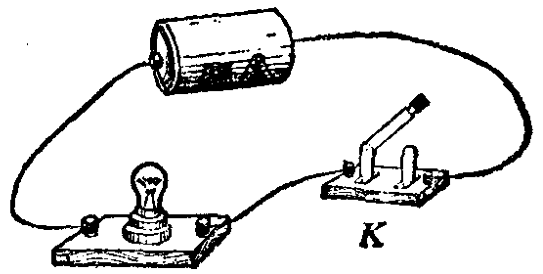
\includegraphics[width=6cm]{../pic/czwl2-ch7-20}
    \caption{}\label{fig:7-20}
\end{wrapfigure}

\xiaobiaoti{电路和电路图}
电灯、电铃、电炉和电动机等利用电流来工作的设备,都叫做用电器。
为了把电流送给用电器,必须用导线把电源和用电器连接起来。
为了随时能够把用电器跟电源连通或者切断,还必须安装开关——电键。

由电源、用电器以及导线、电键等元件组成的电流路径,叫做\textbf{电路}。
图 \ref{fig:7-20} 就是一个简单的电路。
在这个电路中,干电池是电源,小灯泡是用电器,连接电路用的电线就是导钱,$K$ 是电键。

要使电路中有电流,电路必须是处处连通的,处处连通的电路叫做通路。
如果电路中某处断开了,电路不再闭合,电路中就没有电流了。断开的电路叫做断路。

\begin{figure}[htbp]
    \centering
    \begin{minipage}{11cm}
    \centering
    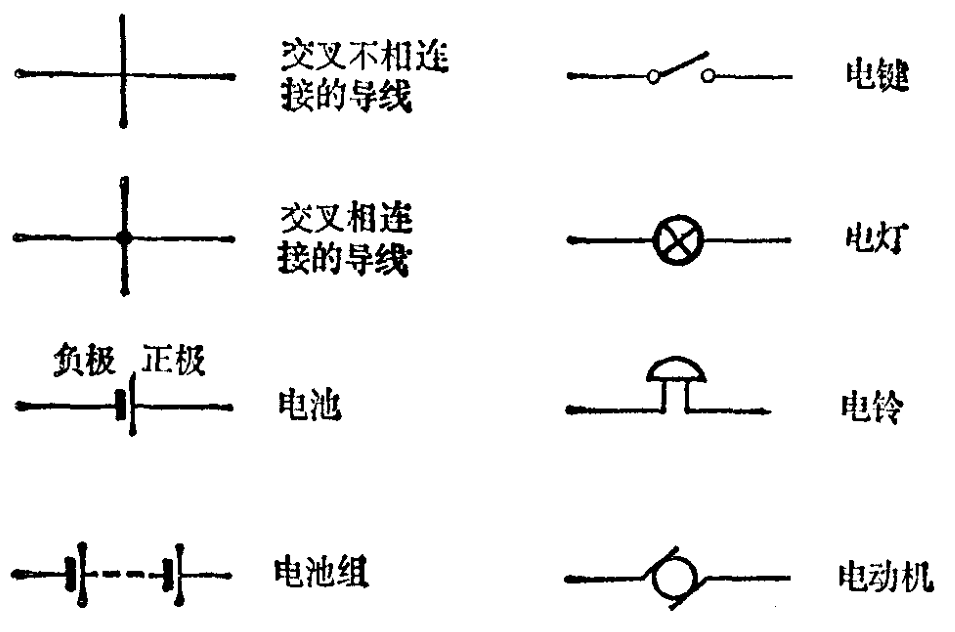
\includegraphics[width=10cm]{../pic/czwl2-ch7-21}
    \caption{几种电路元件的符号}\label{fig:7-21}
    \end{minipage}
    \qquad
    \begin{minipage}{5cm}
    \centering
    \vspace{4cm}
    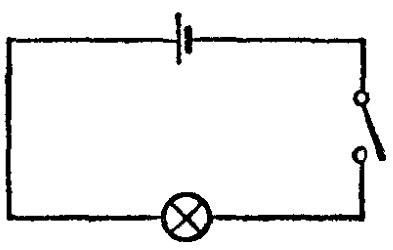
\includegraphics[width=4cm]{../pic/czwl2-ch7-22}
    \caption{}\label{fig:7-22}
    \end{minipage}
\end{figure}


在设计、安装、修理各种实际电路的时候,常常需要画出表示电路连接情况的图。
为了简便,通常不画实物图,而用国家统一规定的符号来代表电路中的各种元件(图 \ref{fig:7-21})。
这种用规定的符号表示电路连接情况的图,叫做电路图。
图 \ref{fig:7-22} 就是图 \ref{fig:7-20} 的电路图。


\xiaobiaoti{串联和并联}
在一个电路里连接的用电器往往不只一个。
如果要在一个电路里连接两盏电灯,有几种连接方法呢?

\begin{figure}[htbp]
    \centering
    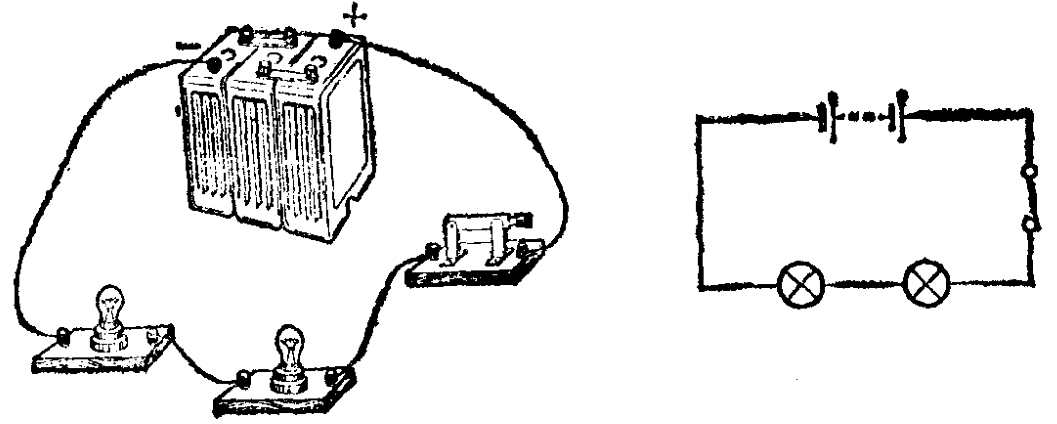
\includegraphics[width=0.7\textwidth]{../pic/czwl2-ch7-23}
    \caption{串联电路}\label{fig:7-23}
\end{figure}

我们可以接照图 \ref{fig:7-23} 那样,把两电灯顺次连接在电路里。
把电路元件逐个顺次连接起来的方法叫做\textbf{串联}。
从图 \ref{fig:7-23} 可以看出,在串联电路里,通过一盏灯的电流也要通过另一盏灯。
如果熄灭一盏电灯(把灯泡从灯座上去掉),电路就被断开,另一盏灯也就不亮了。


我们还可以照图 \ref{fig:7-24} 那样,把两盏电灯并列接在电路的两点间。
把电路元件并列接在电路两点间的连接方法叫做\textbf{并联}。
从图 \ref{fig:7-24} 可以看出,在并联电路里,干路中的电流在分支处分成两部分,
一部分电流通过一盏电灯,另一部分电流通过另一盏电灯。
断开一条支路,这条支路中的电灯就熄灭,
但是另一条支路中的电灯仍旧继续发光,因为它与干路构成的整个电路仍旧是通路。

\begin{figure}[htbp]
    \centering
    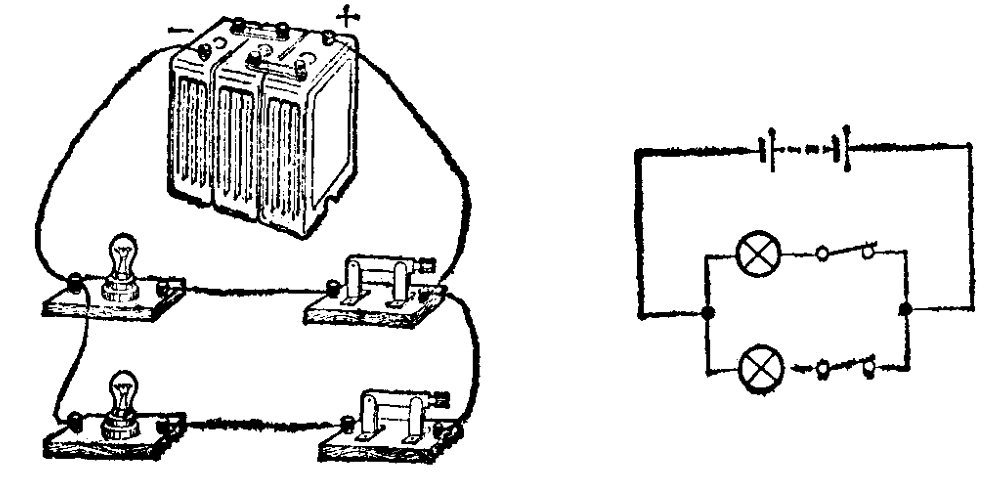
\includegraphics[width=0.7\textwidth]{../pic/czwl2-ch7-24}
    \caption{并联电路}\label{fig:7-24}
\end{figure}


串联和并联是两种最基本的电路连接方法,在实验室里和生产技术中都常常用到。

